% Options for packages loaded elsewhere
\PassOptionsToPackage{unicode}{hyperref}
\PassOptionsToPackage{hyphens}{url}
%
\documentclass[
  ignorenonframetext,
  aspectratio=169]{beamer}
\usepackage{pgfpages}
\setbeamertemplate{caption}[numbered]
\setbeamertemplate{caption label separator}{: }
\setbeamercolor{caption name}{fg=normal text.fg}
\beamertemplatenavigationsymbolsempty
% Prevent slide breaks in the middle of a paragraph
\widowpenalties 1 10000
\raggedbottom
\setbeamertemplate{part page}{
  \centering
  \begin{beamercolorbox}[sep=16pt,center]{part title}
    \usebeamerfont{part title}\insertpart\par
  \end{beamercolorbox}
}
\setbeamertemplate{section page}{
  \centering
  \begin{beamercolorbox}[sep=12pt,center]{part title}
    \usebeamerfont{section title}\insertsection\par
  \end{beamercolorbox}
}
\setbeamertemplate{subsection page}{
  \centering
  \begin{beamercolorbox}[sep=8pt,center]{part title}
    \usebeamerfont{subsection title}\insertsubsection\par
  \end{beamercolorbox}
}
\AtBeginPart{
  \frame{\partpage}
}
\AtBeginSection{
  \ifbibliography
  \else
    \frame{\sectionpage}
  \fi
}
\AtBeginSubsection{
  \frame{\subsectionpage}
}
\usepackage{amsmath,amssymb}
\usepackage{iftex}
\ifPDFTeX
  \usepackage[T1]{fontenc}
  \usepackage[utf8]{inputenc}
  \usepackage{textcomp} % provide euro and other symbols
\else % if luatex or xetex
  \usepackage{unicode-math} % this also loads fontspec
  \defaultfontfeatures{Scale=MatchLowercase}
  \defaultfontfeatures[\rmfamily]{Ligatures=TeX,Scale=1}
\fi
\usepackage{lmodern}
\usetheme[]{Montpellier}
\ifPDFTeX\else
  % xetex/luatex font selection
\fi
% Use upquote if available, for straight quotes in verbatim environments
\IfFileExists{upquote.sty}{\usepackage{upquote}}{}
\IfFileExists{microtype.sty}{% use microtype if available
  \usepackage[]{microtype}
  \UseMicrotypeSet[protrusion]{basicmath} % disable protrusion for tt fonts
}{}
\makeatletter
\@ifundefined{KOMAClassName}{% if non-KOMA class
  \IfFileExists{parskip.sty}{%
    \usepackage{parskip}
  }{% else
    \setlength{\parindent}{0pt}
    \setlength{\parskip}{6pt plus 2pt minus 1pt}}
}{% if KOMA class
  \KOMAoptions{parskip=half}}
\makeatother
\usepackage{xcolor}
\newif\ifbibliography
\setlength{\emergencystretch}{3em} % prevent overfull lines
\providecommand{\tightlist}{%
  \setlength{\itemsep}{0pt}\setlength{\parskip}{0pt}}
\setcounter{secnumdepth}{-\maxdimen} % remove section numbering
\AtBeginDocument{\title[Module 1 - Introduction]{\textbf{Environmental and Development Economics} \\ Module 1 - Introduction}}
\input{header.tex}
\ifLuaTeX
  \usepackage{selnolig}  % disable illegal ligatures
\fi
\IfFileExists{bookmark.sty}{\usepackage{bookmark}}{\usepackage{hyperref}}
\IfFileExists{xurl.sty}{\usepackage{xurl}}{} % add URL line breaks if available
\urlstyle{same}
\hypersetup{
  hidelinks,
  pdfcreator={LaTeX via pandoc}}

\title{Environmental and Development Economics\\
Module 1 - Introduction}
\author{Raahil Madhok\\
UMN Applied Economics}
\date{2026-08-31}

\begin{document}
\frame{\titlepage}

\begin{frame}{Introduce yourself}
\protect\hypertarget{introduce-yourself}{}
\begin{itemize}
\item
  First, lets do introductions \vfill
\item
  Name, year, memorable summer activity, \textbf{research interests}
  \vfill
\item
  Why are you taking this class?
\end{itemize}
\end{frame}

\begin{frame}{Housekeeping}
\protect\hypertarget{housekeeping}{}
\begin{itemize}
\tightlist
\item
  \textbf{Class Time/Location:} Mon/Wed 8:45am-10:25pm, Ruttan B42

  \begin{itemize}
  \tightlist
  \item
    Last class: Oct 26th
  \end{itemize}
\end{itemize}

\vfill

\begin{itemize}
\tightlist
\item
  \textbf{Office Hours:} Tues/Thurs 12:00pm-1:00pm, Ruttan 337D \vfill
\item
  \textbf{Course website:}
  \url{https://github.com/rmadhok/enviro-dev-grad}

  \begin{itemize}
  \tightlist
  \item
    lectures, assignments, syllabus
  \item
    Try to skim reading(s) beforehand \vfill
  \end{itemize}
\item
  \textbf{Assignments}: Upload through Canvas \vfill
\end{itemize}
\end{frame}

\begin{frame}{Today}
\protect\hypertarget{today}{}
\begin{itemize}
\tightlist
\item
  Why study environmental economics in LMICs? \vfill
\item
  Course overview + detailed outline \vfill
\item
  Grade breakdown \vfill
\item
  If time: conceptual framework for environment \& development econ
\end{itemize}
\end{frame}

\begin{frame}{}
\protect\hypertarget{section}{}
\centering

\huge Why study environmental economics in LMICs?
\end{frame}

\begin{frame}{Why study environmental economics in LMICs?}
\protect\hypertarget{why-study-environmental-economics-in-lmics}{}
\begin{itemize}
\item
  Environmental quality is worse and has worse consequences in LMICs

  \begin{itemize}
  \tightlist
  \item
    Highest pollution, highest deforestation
  \end{itemize}
\item
  New field: room for applied theory, empirical innovation
\item
  Data breakthroughs

  \begin{itemize}
  \tightlist
  \item
    Measurement: remote sensing, DHS, etc.
  \item
    Access: lower barriers to government access and experimentation
  \end{itemize}
\item
  Evidence needed; big implications for poverty alleviation
\end{itemize}
\end{frame}

\begin{frame}{Environmental quality worse in LMICs}
\protect\hypertarget{environmental-quality-worse-in-lmics}{}
\begin{center}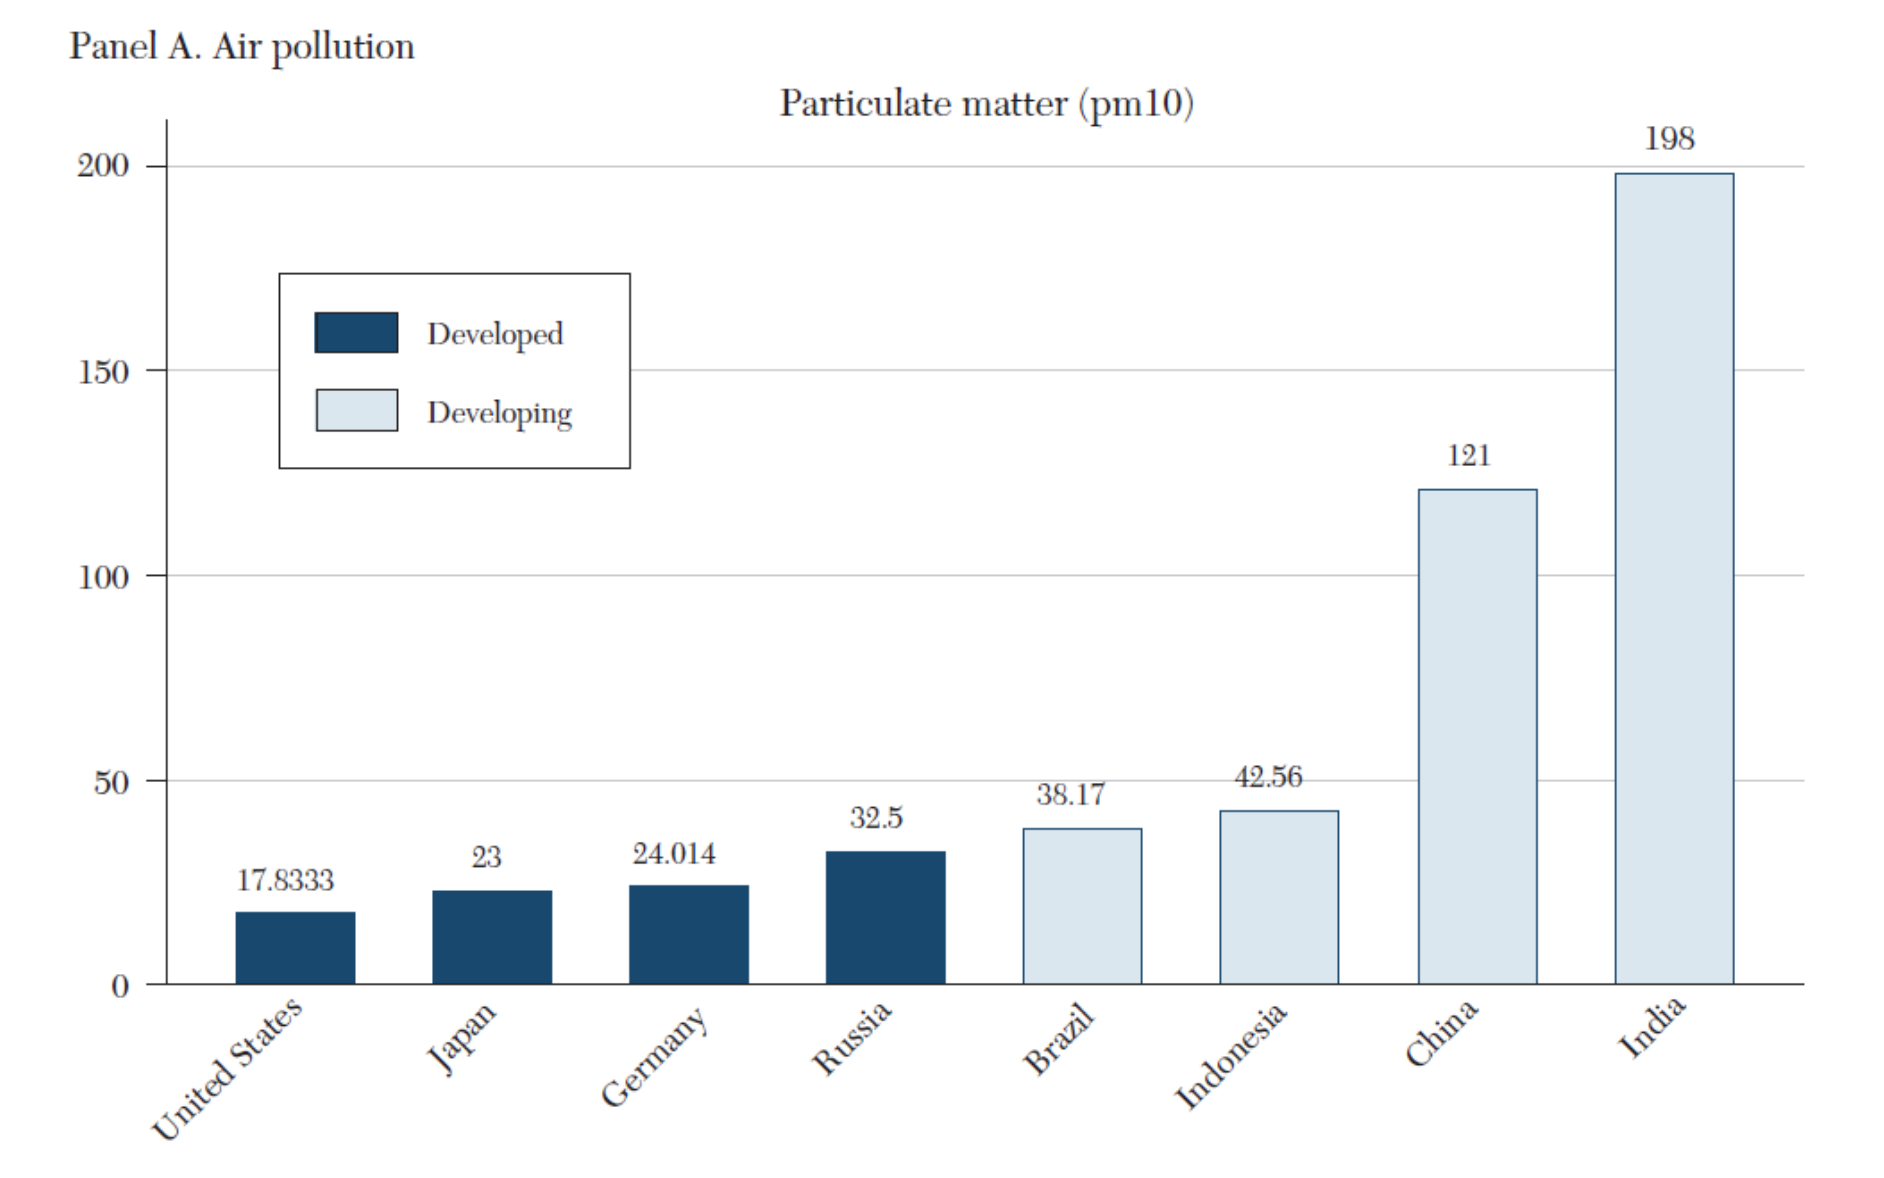
\includegraphics[width=0.85\linewidth]{assets/pm_lmic} \end{center}
\end{frame}

\begin{frame}{Disease burden higher in LMICs}
\protect\hypertarget{disease-burden-higher-in-lmics}{}
\begin{center}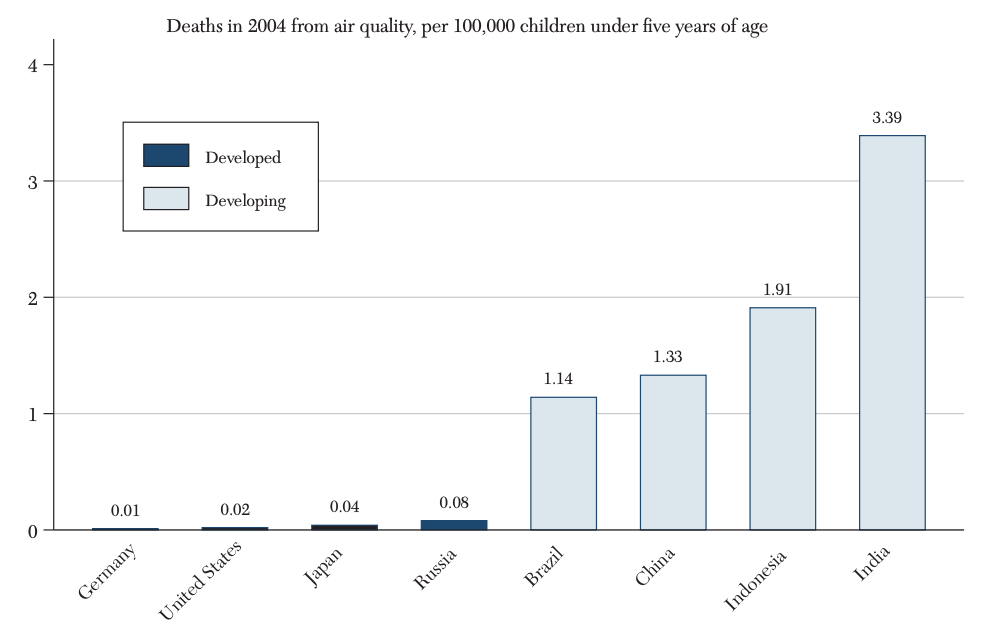
\includegraphics[width=0.85\linewidth]{assets/disease_lmic} \end{center}
\end{frame}

\begin{frame}{Is environmental economics different in LMICs?}
\protect\hypertarget{is-environmental-economics-different-in-lmics}{}
My answer: sometimes\ldots{} \vfill 

\begin{itemize}
\item
  Magnitudes

  \begin{itemize}
  \tightlist
  \item
    Same questions, but costs and benefits different
  \end{itemize}
\item
  \textbf{Local} environmental quality is more important
\item
  Different topics

  \begin{itemize}
  \tightlist
  \item
    cookstoves, enforcement/corruption, ethnic favoritism
  \end{itemize}
\item
  Institutions and state capacity
\end{itemize}
\end{frame}

\begin{frame}{}
\protect\hypertarget{section-1}{}
\centering

\huge Course Overview
\end{frame}

\begin{frame}{Course Overview: There is no textbook}
\protect\hypertarget{course-overview-there-is-no-textbook}{}
Instead, I am organizing around \textbf{\textcolor{orange}{FIVE}} key
questions:

\begin{enumerate}
\item
  How does economic development affect the environment, and vice versa?
\item
  Why is environmental quality so bad in developing countries?
\item
  What are the costs of poor environmental quality in developing
  countries?
\item
  Why is WTP for environmental quality low in developing countries?
\item
  What are the political economy barriers to environmental protection?
\end{enumerate}
\end{frame}

\begin{frame}{Course Approach}
\protect\hypertarget{course-approach}{}
I will:

\begin{itemize}
\item
  Frame (almost) each topic with some theory
\item
  Teach applied papers

  \begin{itemize}
  \tightlist
  \item
    research design, identification strategy, estimation techniques
  \item
    aim for two per class (please skim beforehand)
  \end{itemize}
\item
  Emphasize recent papers
\end{itemize}

\vfill

I will NOT:

\begin{itemize}
\item
  Teach econometrics
\item
  Teach coding
\item
  Teach every topic in environment/development
\end{itemize}
\end{frame}

\begin{frame}{Course Goals}
\protect\hypertarget{course-goals}{}
\begin{enumerate}
\item
  Show you environment/development research frontier
\item
  Inspire your thesis/JMP ideas
\item
  Advance your training as applied microeconomists
\item
  Show you what makes a top-tier research question
\end{enumerate}
\end{frame}

\begin{frame}{Course Structure}
\protect\hypertarget{course-structure}{}
\begin{itemize}
\tightlist
\item
  This is a brand new class, so I give myself leeway to make changes
  \vfill
\item
  You have the unique opportunity to determine direction of the course

  \begin{itemize}
  \tightlist
  \item
    Think about what topics do and don't interest you
  \item
    And let me know! \vfill
  \end{itemize}
\item
  Please check the course website regularly for updates
\end{itemize}
\end{frame}

\begin{frame}{}
\protect\hypertarget{section-2}{}
\centering

\huge Course Outline and Topics
\end{frame}

\begin{frame}{Course Outline}
\protect\hypertarget{course-outline}{}
\textbf{Module 1: Introduction}

\begin{itemize}
\tightlist
\item
  Lecture 1: Course intro + how to use theory to ask the right questions
\end{itemize}

\vfill

\textbf{Module 2: The effect of development on the environment}

\begin{itemize}
\tightlist
\item
  Lecture 2: Income effects
\item
  Lecture 3: Access to capital (technology and infrastructure)
\end{itemize}
\end{frame}

\begin{frame}{Course Outline}
\protect\hypertarget{course-outline-1}{}
\textbf{Module 3: The effect of environment on development}

\begin{itemize}
\tightlist
\item
  Lecture 4: Health
\item
  Lecture 5: Productivity \vfill
\end{itemize}

\textbf{Module 4: Why is WTP low in developing countries?}

\begin{itemize}
\tightlist
\item
  Lecture 6: Revealed preference approaches
\item
  Lecture 7: Incentive compatible approaches
\end{itemize}
\end{frame}

\begin{frame}{Course Outline}
\protect\hypertarget{course-outline-2}{}
\textbf{Module 5: Environmental Policy Design}

\begin{itemize}
\tightlist
\item
  Lecture 8: Monitoring, enforcement
\item
  Lecture 9: Barriers to optimal design \vfill
\end{itemize}

\textbf{Module 6: Political Economy of the Environment}

\begin{itemize}
\tightlist
\item
  Lecture 10: Electoral cycles, corruption
\item
  Lecture 11: State Capacity
\end{itemize}
\end{frame}

\begin{frame}{Course Outline}
\protect\hypertarget{course-outline-3}{}
\textbf{Module 7: Research Proposal Presentations}

\begin{itemize}
\tightlist
\item
  Lecture 12: TBD
\item
  Lecture 13: Presentations
\item
  Lecture 14: Presentations
\end{itemize}
\end{frame}

\begin{frame}{}
\protect\hypertarget{section-3}{}
\centering

\huge Grade Breakdown
\end{frame}

\begin{frame}{Breakdown}
\protect\hypertarget{breakdown}{}
\Large

\begin{table}[]
\begin{tabular}{lllll}
In-class presentations      & 10\% &  &  &  \\
Replication Assignment           & 20\% &  &  &  \\
Research Proposal & 60 \% &  &  &  \\
Participation                     & 10\%     &  &  & 
\end{tabular}
\end{table}
\end{frame}

\begin{frame}{In-class presentations (10\%)}
\protect\hypertarget{in-class-presentations-10}{}
\begin{itemize}
\item
  I want you to become expert presenters after taking this class
\item
  At start of \textbf{each} class, you'll give a 10 min paper
  presentation

  \begin{itemize}
  \tightlist
  \item
    The paper for presentation is on the syllabus
  \end{itemize}
\item
  You will submit \textbf{10} summary slides (5\% of grade)

  \begin{itemize}
  \tightlist
  \item
    motivation, research question, methods, results
  \item
    You may use AI
  \item
    You can submit slides as a group of up to four
  \item
    10 mins presentation + 5 mins Q\&A (5\% of grade)
  \end{itemize}
\item
  I will select presenter on-the-spot

  \begin{itemize}
  \tightlist
  \item
    \textbf{randomly} with replacement**
  \end{itemize}
\end{itemize}

\vfill

** \footnotesize If you are never chosen, your grade is based on slides.
\end{frame}

\begin{frame}{Problem Set (20\%)}
\protect\hypertarget{problem-set-20}{}
\begin{itemize}
\item
  You will replicate an environment/development paper

  \begin{itemize}
  \tightlist
  \item
    You will also \textbf{extend} the results
  \item
    Many papers on the syllabus have replication files
  \end{itemize}
\item
  You will submit a write-up explaining what you did
\item
  You will become familiar with coding in publication-quality papers
\item
  You will use R or Stata
\end{itemize}
\end{frame}

\begin{frame}{Research Proposal (60\%)}
\protect\hypertarget{research-proposal-60}{}
\begin{table}[]
\begin{tabular}{lllll}
Written Proposal      & 30\% & Oct. 30  &  &  \\
First Draft      & pass/fail \% & Oct. 5th  &  &  \\
Peer Review           & 20\% & Oct. 14th  &  &  \\
Proposal Presentation & 10\% & Oct 21/26  &  &  \\
                      &      &  &  & 
\end{tabular}
\end{table}

\begin{itemize}
\item
  You will develop a research proposal for an original idea

  \begin{itemize}
  \tightlist
  \item
    You are NOT expected to actually do the analysis\\
  \item
    I will provide small deadlines (first draft, etc.) along the way
  \end{itemize}
\item
  Come to office hours to pitch your idea
\item
  You will peer review each others proposals
\item
  You will present the proposal at the end of the semester (20 mins)
\end{itemize}
\end{frame}

\begin{frame}{Participation (10\%)}
\protect\hypertarget{participation-10}{}
\begin{itemize}
\item
  I take this seriously
\item
  Not enough to just show up to class
\item
  Quality of questions/discussion count

  \begin{itemize}
  \tightlist
  \item
    Office hours/emails also count
  \end{itemize}
\end{itemize}
\end{frame}

\begin{frame}{}
\protect\hypertarget{section-4}{}
\centering

\Huge Questions?
\end{frame}

\begin{frame}{Today}
\protect\hypertarget{today-1}{}
\begin{itemize}
\tightlist
\item
  \textbf{Guiding question:} Why is environmental quality so low in
  LMICs?
\end{itemize}

\vfill

\begin{itemize}
\tightlist
\item
  Your explanations
\end{itemize}

\vfill

\begin{itemize}
\tightlist
\item
  \textbf{Main goal:} Conceptual framework

  \begin{itemize}
  \tightlist
  \item
    Four \emph{theory-informed explanations}
  \item
    Set the stage for rest of class
  \end{itemize}
\end{itemize}

\vfill
\end{frame}

\begin{frame}{Remember from last time}
\protect\hypertarget{remember-from-last-time}{}
\begin{center}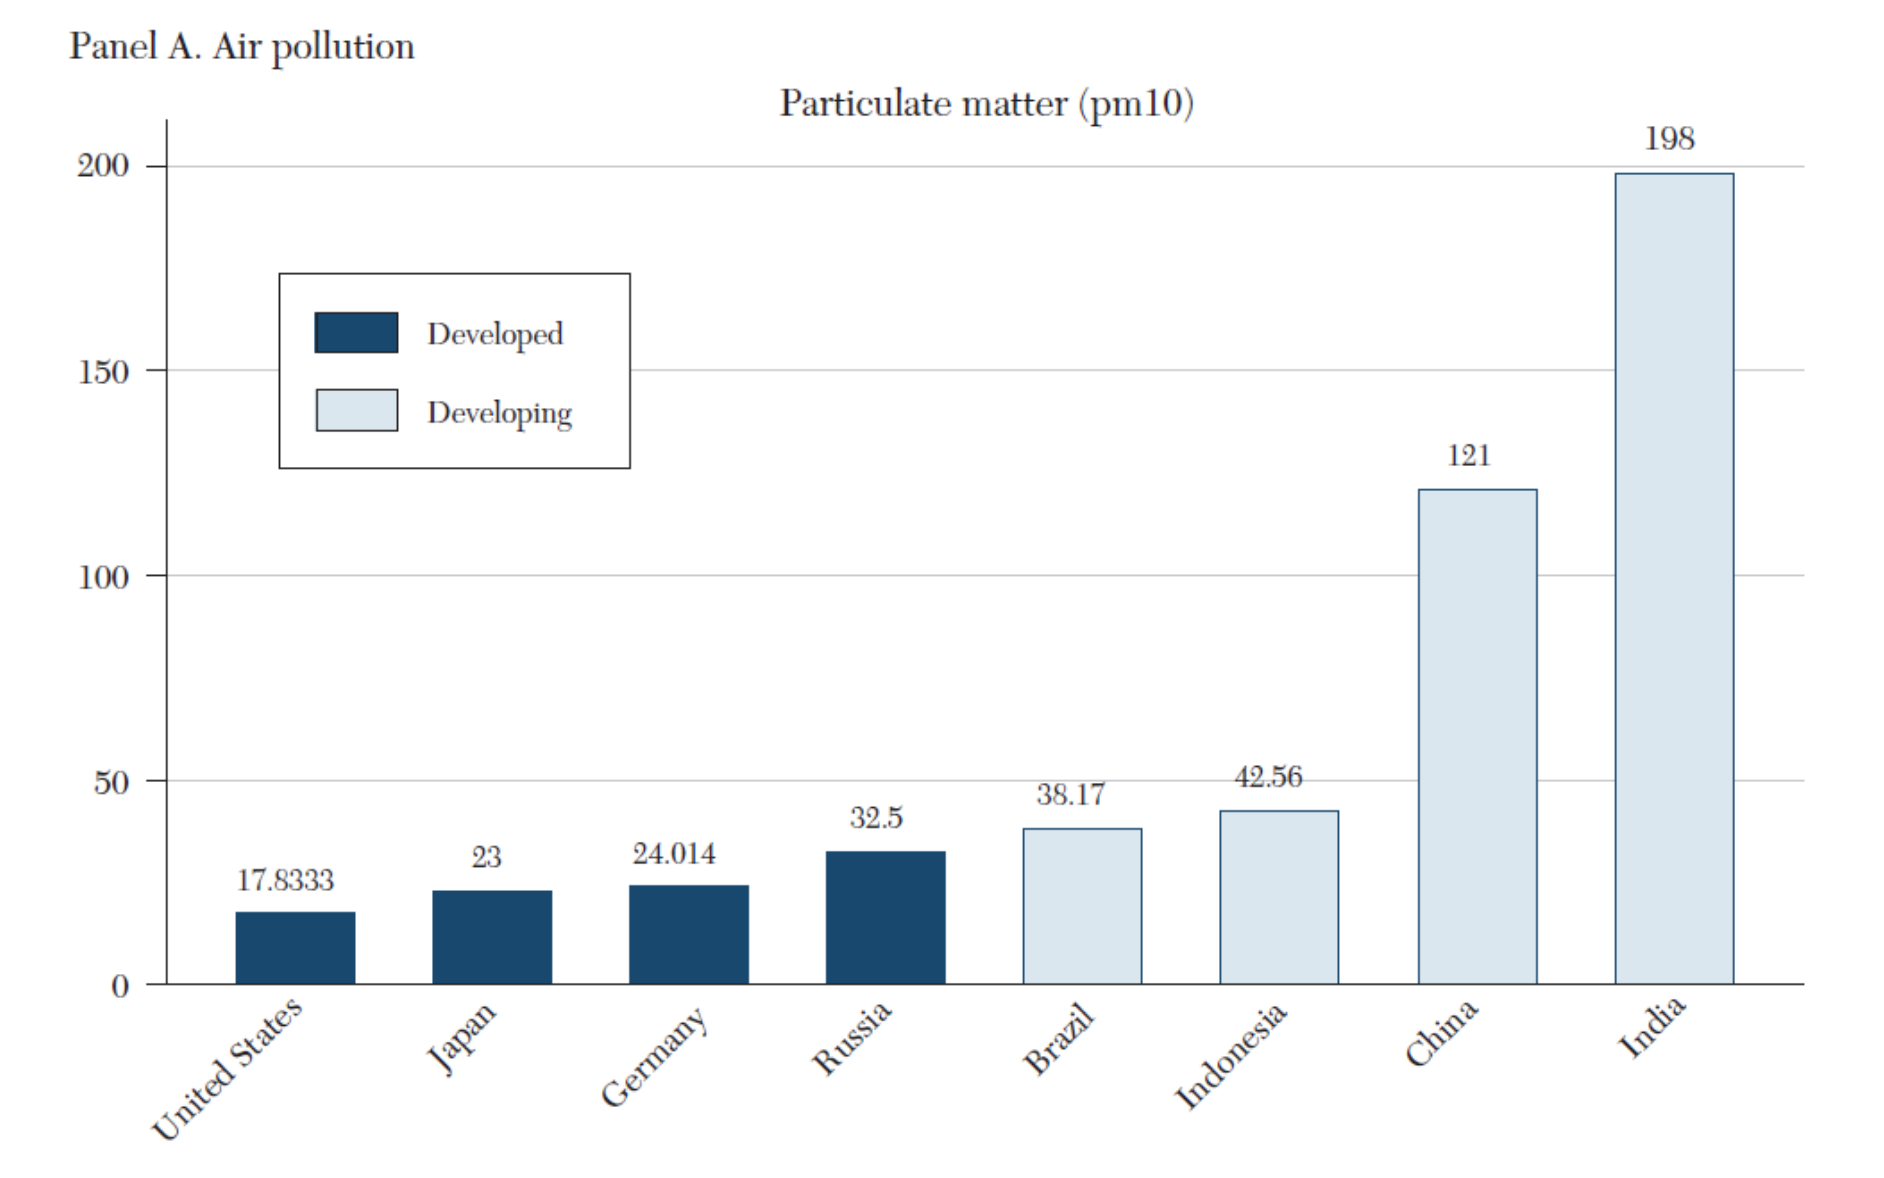
\includegraphics[width=0.85\linewidth]{assets/pm_lmic} \end{center}
\end{frame}

\begin{frame}{Remember from last time}
\protect\hypertarget{remember-from-last-time-1}{}
\begin{center}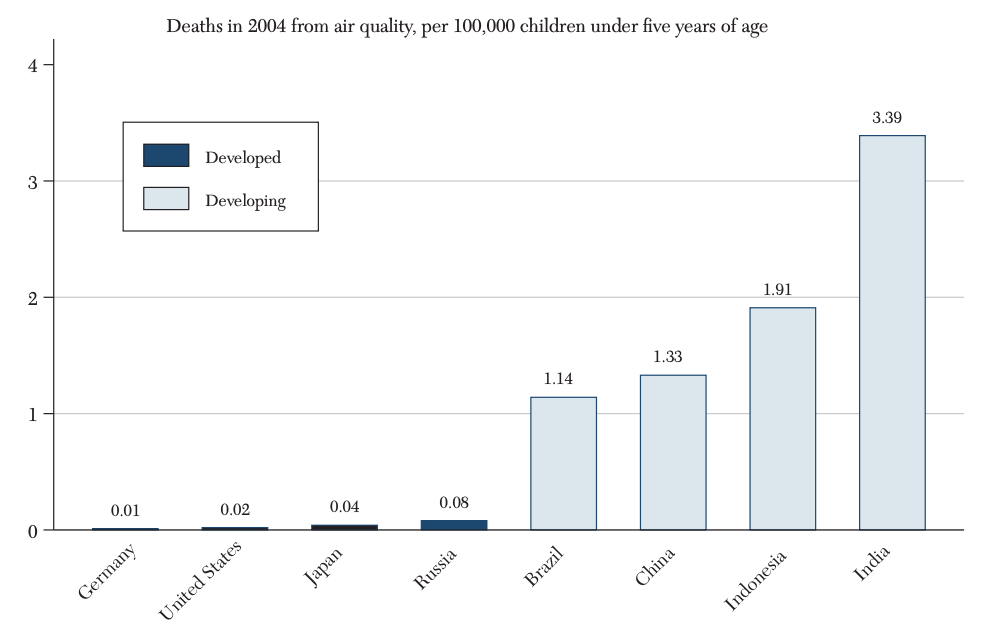
\includegraphics[width=0.85\linewidth]{assets/disease_lmic} \end{center}
\end{frame}

\begin{frame}{Why is environmental quality low in LMICs?}
\protect\hypertarget{why-is-environmental-quality-low-in-lmics}{}
\begin{itemize}
\item
  MWTP is low (paradox)

  \begin{itemize}
  \tightlist
  \item
    Berkouwer and Dean (2022): \$12 for clean air
  \item
    Kremer et al.~(2013): \textasciitilde{} \$4 for clean water

    \begin{itemize}
    \tightlist
    \item
      Imply VSL \$USD 860 vs \$USD 8.6 million for USA
    \end{itemize}
  \end{itemize}
\item
  Do we take this as given? Perhaps status quo is optimal

  \begin{itemize}
  \tightlist
  \item
    is bad environmental quality another dimension of poverty?
  \end{itemize}
\item
  Is welfare loss from pollution greater in rich countries, even though
  they're cleaner?
\item
  \textbf{What are your explanations?}
\end{itemize}
\end{frame}

\begin{frame}{}
\protect\hypertarget{section-5}{}
\centering

\Huge Theory-informed Explanations

\large Greenstone and Jack (2013)
\end{frame}

\begin{frame}{Aside: why is applied theory important?}
\protect\hypertarget{aside-why-is-applied-theory-important}{}
\begin{itemize}
\item
  Builds structure for answering big (and small) questions
\item
  Generates potentially unexpected insights w/ testable predictions
\item
  In reverse: helps rationalize results
\item
  Gets you into better journals (and better jobs)
\item
  Field is headed that way (from my recent experience)
\end{itemize}
\end{frame}

\begin{frame}{Conceptual Framework of Environmental and Development
Economics}
\protect\hypertarget{conceptual-framework-of-environmental-and-development-economics}{}
\begin{itemize}
\tightlist
\item
  Social planner chooses optimal EQ where social \(MWTP_{e} = MC\)

  \begin{itemize}
  \tightlist
  \item
    Need to know MWTP for representative agent
  \end{itemize}
\end{itemize}

\vfill

Set up:

\begin{itemize}
\tightlist
\item
  \(n\) identical agents with utility from consumption, EQ, and health
\item
  Initial individual wealth \(y_{0}\), health \(h_{0}\), environmental
  equality \(e_{0}\)
\item
  health depends on self-protection, \(s\), and \(e\)
\item
  Assume perfect markets (i.e.~no externalities) to benchmark first-best
\end{itemize}
\end{frame}

\begin{frame}{First Best}
\protect\hypertarget{first-best}{}
\begin{itemize}
\tightlist
\item
  Agent chooses \(c\), \(\Delta e\), and \(s\) to maximize:
\end{itemize}

\[ U(e, h(s,e), c) \quad \quad \text{s.t.} \quad \quad y \geq c_{e}(\Delta e) + c_{s}(s) + c\]

\begin{itemize}
\item
  where wealth (endowment + income) and experienced EQ are:
  \[y = y_{0} + \Delta y(e, h(s, e))\]
  \[e = e_{0} + \Delta e + a(c, s)\]
\item
  where \(a(c, s)\) captures impact of \(c\) and \(s\) on EQ
\end{itemize}
\end{frame}

\begin{frame}{Model Particulars}
\protect\hypertarget{model-particulars}{}
\begin{itemize}
\tightlist
\item
  EQ affects utility directly through existence value \vfill
\item
  EQ affects utility indirectly via health (which also affects income)

  \begin{itemize}
  \tightlist
  \item
    e.g.~pollution exposure affects productivity
  \item
    This can be mitigated by self-protection, \(s\) (e.g.~mask, air
    purifier) \vfill
  \end{itemize}
\item
  EQ affects income, which in turn affects utility via budget constraint

  \begin{itemize}
  \tightlist
  \item
    e.g.~agricultural productivity \vfill
  \end{itemize}
\item
  Experienced EQ depends directly on \(\Delta e\), and indirectly via
  \(c\), \(s\)

  \begin{itemize}
  \tightlist
  \item
    \(a(c,s)\): defensive investments i.e.~clean cookstove, bottled
    water, etc.
  \end{itemize}
\end{itemize}
\end{frame}

\begin{frame}{MWTP for improving environmental quality}
\protect\hypertarget{mwtp-for-improving-environmental-quality}{}
\begin{itemize}
\item
  Let \(\lambda_{e} = \frac{\partial u}{\partial \Delta e}\),
  \(\lambda_{y} = \frac{\partial u}{\partial c}\)
\item
  Set up lagrangian and solve for \(MWTP_{e}\): \begin{align}
  MWTP_{e} = \frac{\lambda_{e}}{\lambda_{y}} 
   = \frac{1}{\lambda_{y}} \left(\frac{\partial u}{\partial e} + \frac{\partial u}{\partial h}\frac{\partial h}{\partial e}\right) + \frac{\partial \Delta y}{\partial e} + \frac{\partial \Delta y}{\partial h}\frac{\partial h}{\partial e} \notag
  \end{align}
\item
  aesthetic benefit from improved EQ (converted to dollars)
\item
  indirect benefit of EQ for health (converted to dollars)
\item
  direct impact of EQ on income and indirect impact via health \vfill
  \textbf{Note: if \(U''(c)<0\), low \(y \rightarrow\) high MUC
  (\(\lambda_{y}\)) and low \(MWTP_{e}\)}
\end{itemize}
\end{frame}

\begin{frame}{MWTP for self-protection}
\protect\hypertarget{mwtp-for-self-protection}{}
\begin{itemize}
\tightlist
\item
  Set up lagrangian and solve for \(MWTP_{s}\)
\end{itemize}

\begin{align}
MWTP_{s} & = \frac{\lambda_{s}}{\lambda_{y}} \notag \\ & = \frac{1}{\lambda_{y}} \left(\frac{\partial u}{\partial e}\frac{\partial a}{\partial s} + \frac{\partial u}{\partial h} \left(\frac{\partial h}{\partial s} + \frac{\partial h}{\partial e}\frac{\partial a}{\partial s} \right)\right) + \frac{\partial \Delta y}{\partial e}\frac{\partial a}{\partial s} + \frac{\partial \Delta y}{\partial h}\left(\frac{\partial h}{\partial s} + \frac{\partial h}{\partial e}\frac{\partial a}{\partial s}\right) \notag
\end{align}

\begin{itemize}
\tightlist
\item
  indirect effect of \(s\) on EQ and health (converted to dollars)
\item
  indirect effect of \(s\) on income via productivity and health \vfill
  \textbf{Note: if \(U''(c)<0\), high \(y \rightarrow\) low MUC
  (\(\lambda_{y}\)) and high \(MWTP_{s}\)}
\end{itemize}
\end{frame}

\begin{frame}{The Fist Best Outcome}
\protect\hypertarget{the-fist-best-outcome}{}
\begin{itemize}
\tightlist
\item
  Agent sets ratio of marginal costs = ratio of marginal benefits
  \[\frac{MWTP_{e}}{MWTP_{s}}=\frac{\frac{\partial c_{e}}{\partial \Delta e}}{\frac{\partial c_{s}}{\partial \Delta s}}\]
\end{itemize}

\vfill

\begin{itemize}
\tightlist
\item
  For social planner to aggregate over \(n\), we must assume:

  \begin{itemize}
  \tightlist
  \item
    No preferences of her own
  \item
    Can observe true MWTP
  \item
    Anything else? \vfill
  \end{itemize}
\item
  Do these hold in LMICs?
\end{itemize}
\end{frame}

\begin{frame}{Course Structure}
\protect\hypertarget{course-structure-1}{}
\begin{itemize}
\tightlist
\item
  Set the stage:

  \begin{itemize}
  \tightlist
  \item
    how does environment affect development
    (\(\frac{\partial h}{\partial e}\)) (module 2)
  \item
    how does development affect the environment (module 3)
  \end{itemize}
\end{itemize}

\vfill

\begin{itemize}
\tightlist
\item
  Bulk of course:

  \begin{itemize}
  \tightlist
  \item
    Explain why environmental quality low in LMICs
  \item
    Identify as many parameters of the social planner problem as
    possible
  \end{itemize}
\end{itemize}

\vfill

\begin{itemize}
\tightlist
\item
  Goal: where can you make a contribution?

  \begin{itemize}
  \tightlist
  \item
    E.g. Lots of work on \(\frac{\partial h}{\partial e}\), but very
    little on \(\frac{\partial \Delta y}{\partial e}\)
  \end{itemize}
\end{itemize}
\end{frame}

\begin{frame}{Why is environmental quality so low in LMICs?}
\protect\hypertarget{why-is-environmental-quality-so-low-in-lmics}{}
Four explanations informed by the model:

\begin{enumerate}
\item
  High marginal utility of consumption
\item
  High marginal abatement costs -- includes state capacity
\item
  Political economy distortions (first best violation)
\item
  Market failures (first best violation)

  \begin{itemize}
  \tightlist
  \item
    frictions cause revealed MWTP \(\neq\) true MWTP
  \end{itemize}
\end{enumerate}
\end{frame}

\begin{frame}{}
\protect\hypertarget{section-6}{}
\centering

\huge Preview of Answers
\end{frame}

\begin{frame}{1. High marginal utility of consumption}
\protect\hypertarget{high-marginal-utility-of-consumption}{}
\begin{itemize}
\tightlist
\item
  Intuitively, poor people care more about meeting basic consumption
  needs \vfill
\item
  Economically, agent trades off \(c\) and \(e\) by setting
  \(u'(c) = u'(e)\)

  \begin{itemize}
  \tightlist
  \item
    If \(u''(c)<0\), prefer \(c\) at lower levels of \(y\)
  \item
    even if health benefits of \(e\) are large! \vfill
  \end{itemize}
\item
  \textbf{Very} few revealed preference studies on \(MWTP_{e}\)

  \begin{itemize}
  \tightlist
  \item
    Kremer et al.~(2013) randomly clean up springs in Kenya
  \item
    WTP USD 11/year for clean water; VSL of USD 860 \vfill
  \end{itemize}
\item
  Larger literature on \(u'(h)\) also suggests low valuation (Berkouwer
  and Dean, 2022) \vfill
\end{itemize}
\end{frame}

\begin{frame}{2. High MC}
\protect\hypertarget{high-mc}{}
\begin{itemize}
\tightlist
\item
  High MAC suggests sub-optimal environmental quality. Why?

  \begin{itemize}
  \tightlist
  \item
    Upward sloping MAC suggests low MC in poor countries
  \end{itemize}
\end{itemize}

\vfill

\begin{itemize}
\tightlist
\item
  MC not only driven by MAC; also reflects weak state capacity

  \begin{itemize}
  \tightlist
  \item
    Enforcement (Duflo et al., 2013)
  \item
    Incentives (Jagnani and Mahadevan, 2024; Gulzaar and Dipoppa, 2024)
  \item
    Spillovers (Viera et al.~2024)
  \end{itemize}
\end{itemize}

\vfill

\begin{itemize}
\tightlist
\item
  High MC \textbf{does not} mean deviation from first best
\end{itemize}
\end{frame}

\begin{frame}{3. Political economy}
\protect\hypertarget{political-economy}{}
\begin{itemize}
\tightlist
\item
  Social planner includes own utility weights social welfare function

  \begin{itemize}
  \tightlist
  \item
    i.e.~corruption \vfill
  \end{itemize}
\item
  Many examples from LMICs

  \begin{itemize}
  \tightlist
  \item
    pollution (Duflo et al., 2013)
  \item
    deforestation (Burgess et al., 2012)
  \item
    human-wildlife conflict (Madhok et al., 2024) \vfill
  \end{itemize}
\item
  Leads to second best policy (inefficient) \vfill
\end{itemize}
\end{frame}

\begin{frame}{4. Market Failures}
\protect\hypertarget{market-failures}{}
\begin{itemize}
\tightlist
\item
  This is partially a course on development economics

  \begin{itemize}
  \tightlist
  \item
    About market failures: land, labor, credit, etc. \vfill
  \end{itemize}
\item
  Implication for us: revealed \(MWTP_{e} \neq\) first best \(MWTP_{e}\)
  \vfill
\item
  Example: weak property rights \(\rightarrow\) underinvestment in \(e\)

  \begin{itemize}
  \tightlist
  \item
    Underestimate \(MWTP_{e}\) from observed data
  \item
    RCT evidence from crop-burning PES contracts: Jack et al.~(2024)
    \vfill
  \end{itemize}
\end{itemize}
\end{frame}

\begin{frame}{Lots of room for research}
\protect\hypertarget{lots-of-room-for-research}{}
\begin{itemize}
\tightlist
\item
  Environment and development economics is new

  \begin{itemize}
  \tightlist
  \item
    Challenge: find something unique about LMICs \vfill
  \end{itemize}
\item
  Goal: identify model parameters \vfill
\item
  Evidence on many parameters are absent \vfill
\item
  Barriers to research in LMICs are falling

  \begin{itemize}
  \tightlist
  \item
    remote sensing, administrtive/survey data, webscraping \vfill
  \end{itemize}
\end{itemize}
\end{frame}

\begin{frame}{Next Class}
\protect\hypertarget{next-class}{}
\begin{itemize}
\item
  In-class presentations
\item
  Impact of economic development on the environment (income effects)
\item
  Impact of development on the environment (forests, biodiversity)
\end{itemize}
\end{frame}

\begin{frame}{}
\protect\hypertarget{section-7}{}
\huge

Aside: Best Practice for Short Presentations
\end{frame}

\begin{frame}{Best Practices: Structure}
\protect\hypertarget{best-practices-structure}{}
\begin{itemize}
\tightlist
\item
  You cannot present a paper in 10 minutes

  \begin{itemize}
  \tightlist
  \item
    Do not give detailed lit review or go into extreme detail
  \end{itemize}
\end{itemize}

\vfill

\begin{itemize}
\tightlist
\item
  Instead, you are giving a trailer for the movie

  \begin{itemize}
  \tightlist
  \item
    Convince the audience that they should read the paper
  \end{itemize}
\end{itemize}

\vfill

\begin{itemize}
\item
  Your goal is only to state why the paper is important, and what you
  did \vfill
\item
  Convey paper's importance in first slide
\end{itemize}
\end{frame}

\begin{frame}{Best Practices: Slides}
\protect\hypertarget{best-practices-slides}{}
\begin{itemize}
\item
  Motivation + broad research question (1 slide)
\item
  Full paper overview (1 slide)
\item
  Lit review (optional, 1 slide)
\item
  Background (1 slide)
\item
  Data (2 slides)
\item
  Empirical Strategy (2 slides)
\item
  Results (2 slides)
\item
  Summary (1 slide)
\end{itemize}
\end{frame}

\begin{frame}{Example of Preview Slide}
\protect\hypertarget{example-of-preview-slide}{}
\begin{itemize}
\item
  \textbf{Question:} How do firms react to tribal forest policy?
\item
  \textbf{Idea:} Model aggregate economic response and changes in firm
  composition
\item
  \textbf{Setting:} India Forest Rights Act (2008)

  \begin{itemize}
  \tightlist
  \item
    Imposes transaction cost on firms
  \end{itemize}
\item
  \textbf{Data:} Manufacturing census (2001-2015); Deforestation permits
  (2001-2021)
\item
  \textbf{Empirical Strategy:} Diff-in-diff using policy shift in tribal
  and non-tribal district
\end{itemize}

\vfill

\begin{block}{Results Preview}
\protect\hypertarget{results-preview}{}
\begin{enumerate}
[1)]
\tightlist
\item
  decline in firm activity, 2) less forest encroachment by industry\\
\item
  larger, but less productive firms survive
\end{enumerate}
\end{block}
\end{frame}

\begin{frame}{Best Practices: Slide Format}
\protect\hypertarget{best-practices-slide-format}{}
\begin{itemize}
\item
  1 minute per slide
\item
  Avoid chart junk
\item
  One line bullets

  \begin{itemize}
  \tightlist
  \item
    No need for full sentences
  \end{itemize}
\item
  Vary text slides and text + image slides
\item
  Don't put too many equations

  \begin{itemize}
  \tightlist
  \item
    Save details for speaking, or talk ``about'\,' equation
  \end{itemize}
\item
  Summarize findings again at the end
\end{itemize}
\end{frame}

\begin{frame}{Best Practices: Presentation}
\protect\hypertarget{best-practices-presentation}{}
\begin{itemize}
\item
  Speak clearly and loudly
\item
  Speak slowly
\item
  Look at audience; Do not show your back
\item
  Do not stand in front of slides
\item
  Avoid jargon
\item
  Avoid pacing around room
\item
  Stick to your time limit
\end{itemize}
\end{frame}

\end{document}
